%----------------------------------------------------------------------------------------
% БҮЛЭГ 3: АРГ ЗҮЙ БА ДЭВШҮҮЛСЭН САНАА
%----------------------------------------------------------------------------------------

\chapter{Арга зүй ба дэвшүүлсэн санаа}

\section{Системийн архитектур}

Санал болгож буй систем нь \textbf{багш--сурагч загварын мэдлэг дамжуулалт} аргачлал дээр суурилсан бөгөөд видео өгөгдлөөс үйл явдлыг ойлгож, тайлбарлах чадвартай олон төрлийн өгөгдөл боловсруулах том хэлний загварын урсгал юм.

Зурагт системийн ерөнхий архитектурыг үзүүлэв.

% ====================================================================
%  СИСТЕМИЙН АРХИТЕКТУР — цэвэрхэн урсгал TikZ диаграм
% ====================================================================
\begin{figure}[H]
\centering
\resizebox{\linewidth}{!}{%
\begin{tikzpicture}[
  B/.style   = {rectangle, rounded corners=7pt,
                minimum width=4.7cm, minimum height=1.35cm,
                align=center, draw, line width=1pt, font=\small},
  DS/.style  = {B, fill=InputColor!18,   draw=InputColor!70},
  PR/.style  = {B, fill=ProcessColor!18, draw=ProcessColor!70},
  TE/.style  = {B, fill=TeacherColor!18, draw=TeacherColor!70},
  ST/.style  = {B, fill=StudentColor!18, draw=StudentColor!70},
  QA/.style  = {B, fill=DataColor!22,    draw=DataColor!70},
  OU/.style  = {B, fill=OutputColor!18,  draw=OutputColor!70},
  PH/.style  = {rectangle, rounded corners=6pt,
                minimum height=1.0cm, align=center,
                fill=ArrowColor!18, draw=ArrowColor!55, line width=1.2pt,
                font=\small\bfseries, text=ArrowColor!90},
  AR/.style  = {->, >=Stealth, line width=1.1pt, color=ArrowColor!80},
  DR/.style  = {->, >=Stealth, dashed, line width=0.9pt, color=ArrowColor!45},
]

%% ─── ҮЕ ШАТ 1: ӨГӨГДӨЛ БЭЛТГЭХ ──── x = 0 ─────────────────────────────────
\node[PH, minimum width=4.7cm] at (0, 0) (ph1)
  {ҮЕ ШАТ 1 — ӨГӨГДӨЛ БЭЛТГЭХ};

\node[DS, minimum width=4.7cm, below=0.80cm of ph1] (inputs)
  {\textbf{Оролтын өгөгдөл}\\[3pt]
   {\footnotesize RWF-2000 · RLVS · Violence өгөгдлийн багц}\\[-1pt]
   {\footnotesize 1,951 клип / 2,260 тайлбар тайлан}};

\node[PR, minimum width=4.7cm, below=0.65cm of inputs] (prep)
  {\textbf{8-Фрейм Sampling}\\[3pt]
   {\footnotesize $224{\times}224$ фрейм стандартчилал}};

%% ─── ҮЕ ШАТ 2: СУРГАЛТ ──────────── x = 7.0 ─────────────────────────────
\node[PH, minimum width=5.3cm] at (8.5, 0) (ph2)
  {ҮЕ ШАТ 2 — СУРГАЛТ};

\node[TE, minimum width=5.3cm, below=0.80cm of ph2] (te)
  {\textbf{Багш: Qwen3-VL-30B-A3B}\\[3pt]
   {\footnotesize MoE · 3.7B идэвхтэй / 30B нийт · 62.2 GB VRAM}};

    \node[QA, minimum width=5.3cm, below=0.65cm of te] (qa)
      {\textbf{Q\&A Өгөгдлийн багц}\\[3pt]
       {\footnotesize $\sim$9{,}040 хос}};

\node[ST, minimum width=5.3cm, below=0.65cm of qa] (st)
  {\textbf{Сурагч: Qwen2.5-VL-7B}\\[3pt]
   {\footnotesize нарийвчилсан тохируулгатай сурагч загвар}};

    \node[PR, minimum width=5.3cm, below=0.65cm of st] (tr)
      {\textbf{Сурагч загварын сургалт}\\[3pt]
       {\footnotesize Q\&A өгөгдөл · $\approx$40 цаг · A100}};

\node[QA, minimum width=5.3cm, below=0.60cm of tr] (hf)
  {\textbf{HuggingFace Hub}\\[3pt]
   {\footnotesize \texttt{stillmeta/fight-video-qlora1}}};

%% ─── ҮЕ ШАТ 3: INFERENCE ────────────── x = 14.5 ────────────────────────────
\node[PH, minimum width=4.7cm] at (17.0, 0) (ph3)
  {ҮЕ ШАТ 3 — INFERENCE};

\node[DS, minimum width=4.7cm, below=0.80cm of ph3] (vi)
  {\textbf{Видео Оролт}\\[3pt]
   {\footnotesize хяналтын камерын бичлэг}};

\node[ST, minimum width=4.7cm, below=0.65cm of vi] (fm)
  {\textbf{Нарийвчилсан тохируулсан Qwen2.5-7B}\\[3pt]
   {\footnotesize LoRA merged}};

\node[OU, minimum width=4.7cm, minimum height=2.5cm,
      below=0.65cm of fm] (out)
  {\textbf{Монгол Тайлан}\\[0.22cm]
   {\footnotesize Шошго · Итгэлцэл · Субъект}\\[0pt]
   {\footnotesize Явц (T0–T3) · Нотлох баримт}\\[0pt]
   {\footnotesize Дүгнэлт · Зөвлөмж}};

%% ─── ВЕБ UI ДЭЛГЭЦ ──────────────────────────────────────────────────────────
\node[right=1.9cm of fm, inner sep=3pt,
      draw=OutputColor!65, rounded corners=5pt,
      fill=white, line width=1.1pt] (webui)
  {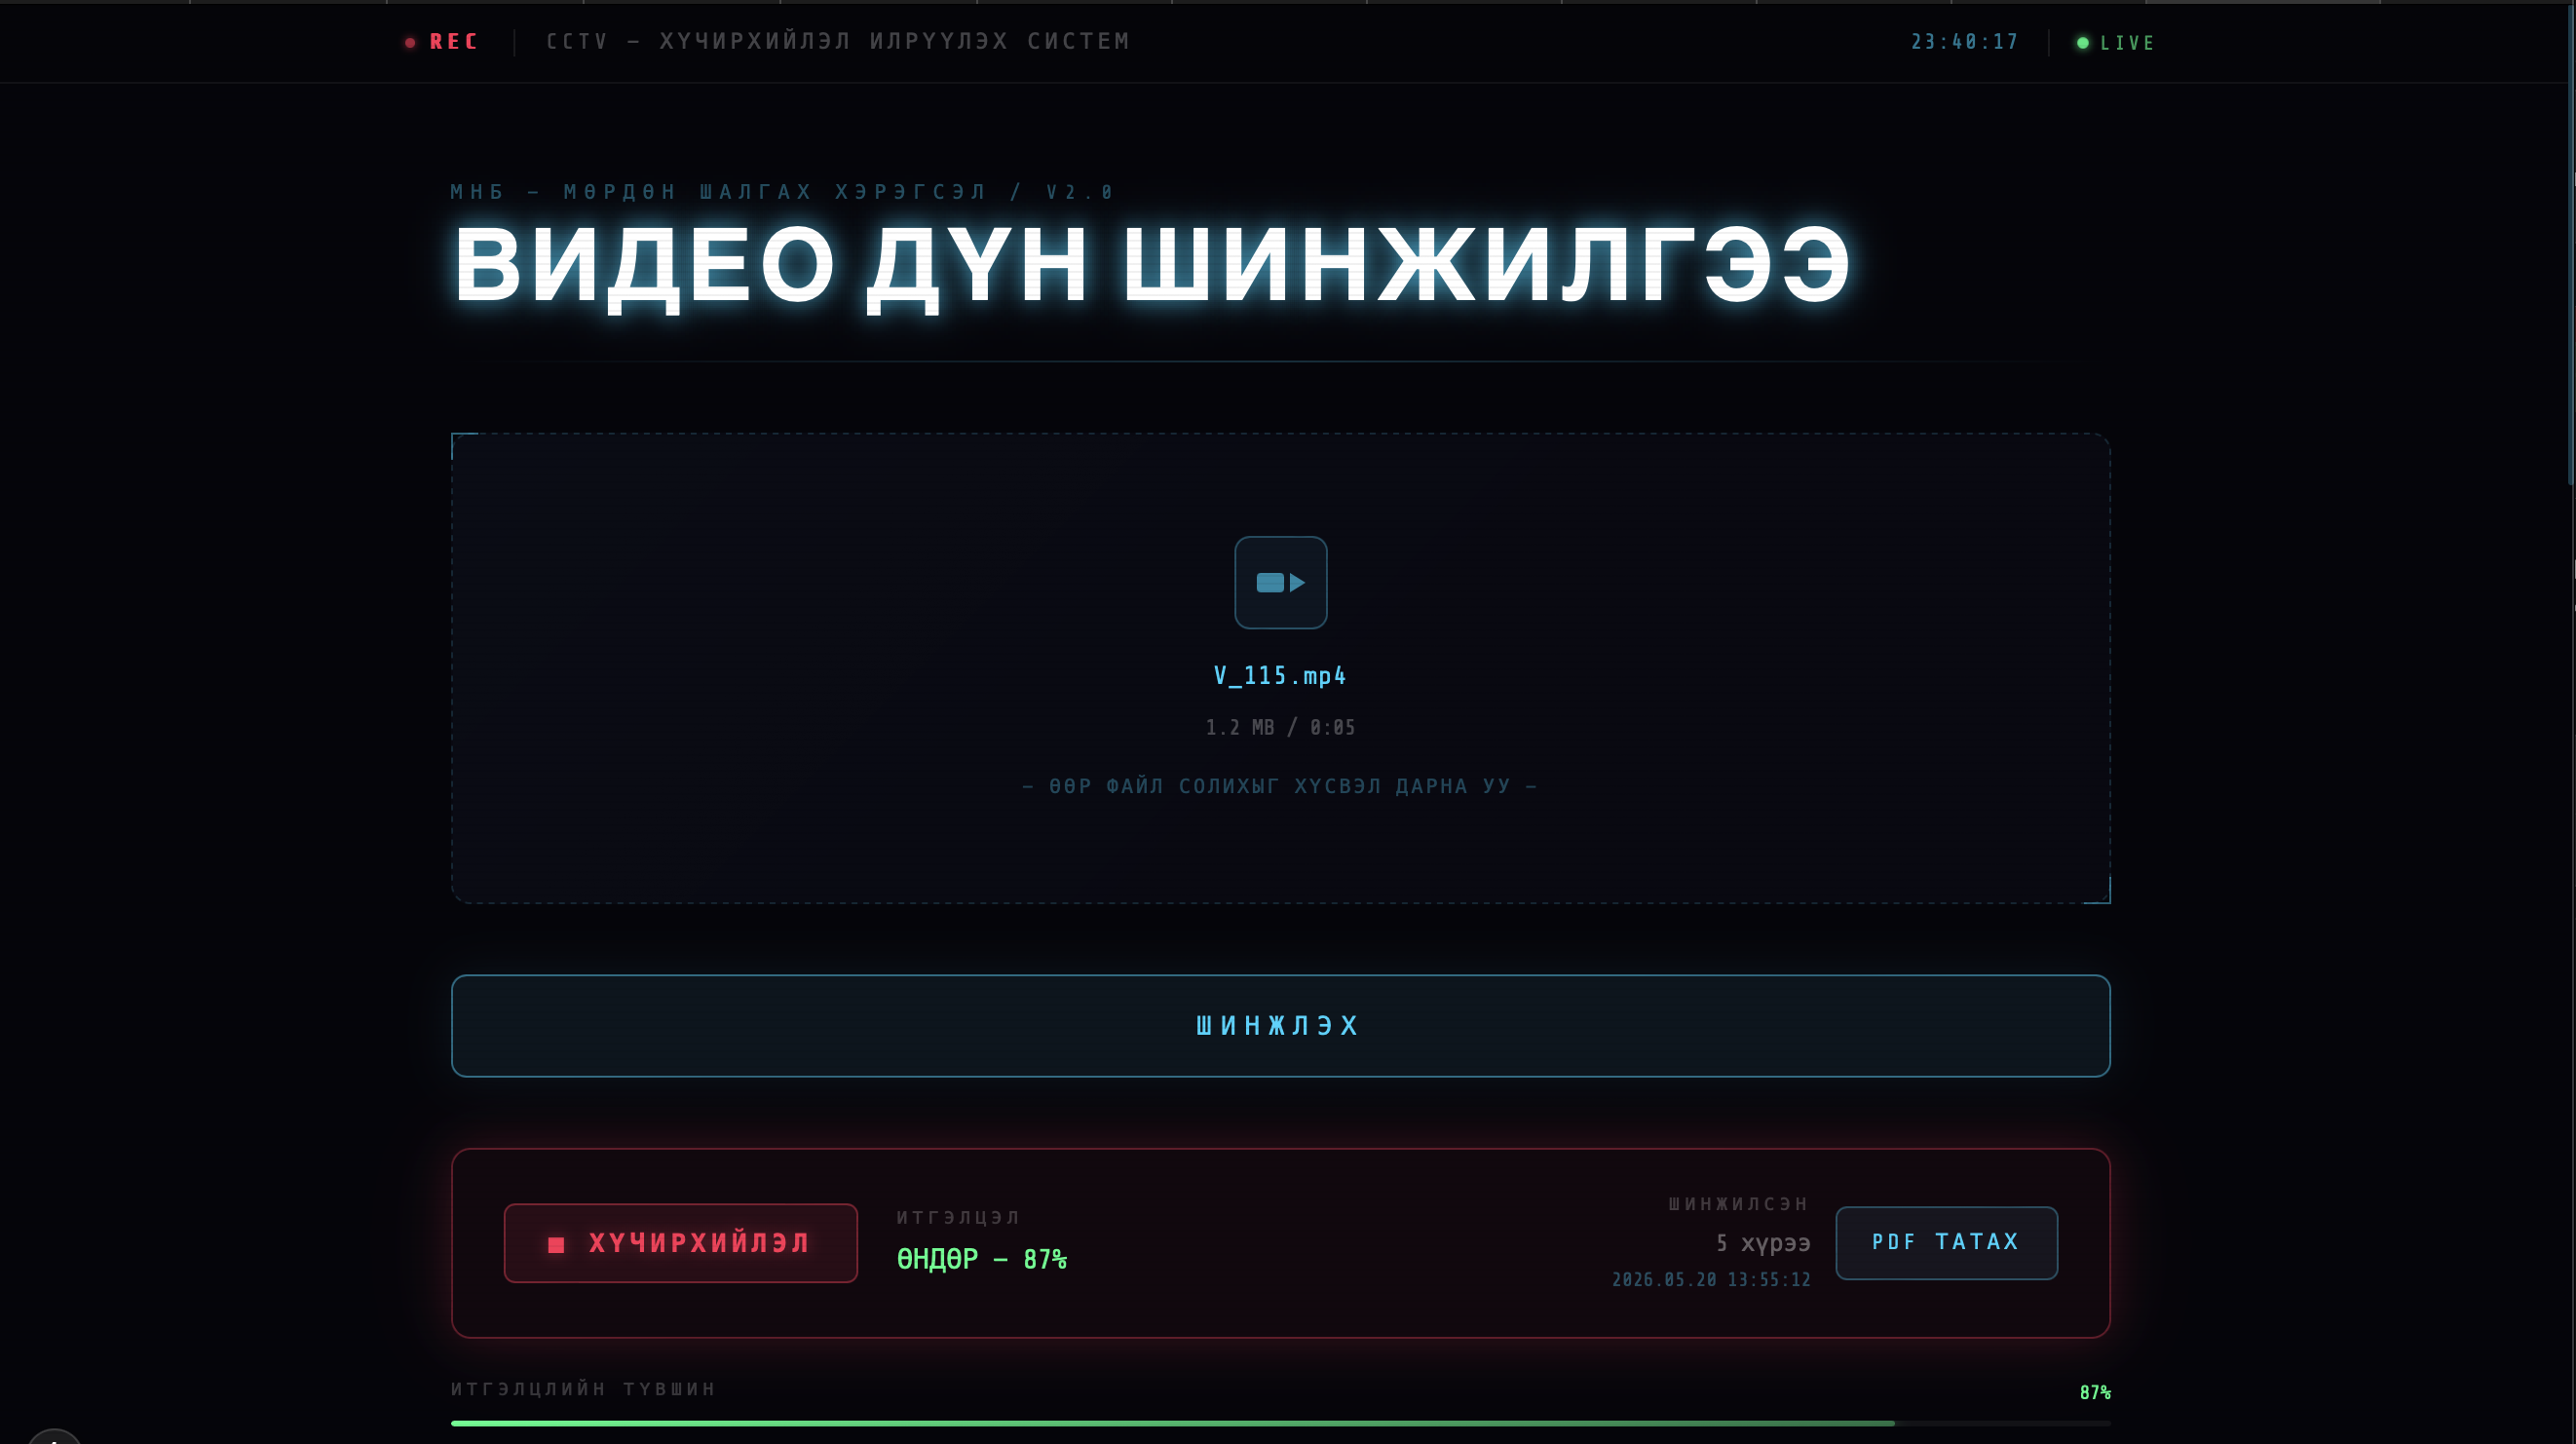
\includegraphics[width=5.6cm]{Figures/web_ui}};
\node[above=4pt of webui, font=\small\bfseries, text=ArrowColor!85]
  {Веб UI демо};

%% ─── СУМНУУД ─────────────────────────────────────────────────────────────────

% P1 internal
\draw[AR] (inputs) -- (prep);

% P1 → P2
\draw[AR] (prep.east) -- ++(0.5,0) |- (te.west);

% P2 internal
\draw[AR] (te) -- (qa);
\draw[AR] (qa) -- (st);
\draw[AR] (st) -- (tr);
\draw[DR] (tr) -- (hf);

% P2 → P3
\draw[AR] (tr.east) -- ++(0.65,0) |- (fm.west);

% P3 internal
\draw[AR] (vi) -- (fm);
\draw[AR] (fm) -- (out);

% fm → Web UI
\draw[DR] (fm.east) -- (webui.west)
  node[midway, above=3pt, font=\scriptsize\itshape, text=OutputColor!75]
  {Web UI};

%% ─── ФАЗ ТУСГААРЛАХ ШУГАМ ───────────────────────────────────────────────────
\draw[black!18, dashed, line width=0.7pt]
  ($(ph1.north east)!0.5!(ph2.north west)$) ++(0,0.5) -- ++(0,-13.5);
\draw[black!18, dashed, line width=0.7pt]
  ($(ph2.north east)!0.5!(ph3.north west)$) ++(0,0.5) -- ++(0,-13.5);

\end{tikzpicture}%
}
\caption{Системийн архитектур}
\label{fig:system_урсгал}
\end{figure}

\subsection{Зурагт үзүүлсэн архитектурын тайлбар}

Зургийн дунд хэсэгт \textbf{сурагч загварын сургалт} үе шат байна. Суурь загвар Qwen2.5-VL-7B-ийг бэлтгэсэн Q\&A өгөгдлөөр нарийвчлан тохируулж, сургалтын явцын үзүүлэлтүүдийг WandB-д хөтөлнө. Сургалт дууссаны дараа загварын жинг HuggingFace Hub-т байршуулна.

Зургийн баруун хэсэгт \textbf{дүгнэлт гаргалтын} үе шат байна. Туршилтын видеоноос 8 кадр гарган авч, нарийн тохируулсан загварт дамжуулна. Загвар нь Монгол хэл дээр ШОШГО, ИТГЭЛЦЭЛ, СУБЪЕКТҮҮД, ҮЙЛДЛҮҮД, ЯВЦ, НОТЛОХ БАРИМТ, ДҮГНЭЛТ, ЗӨВЛӨМЖ гэсэн 8 хэсэгтэй бүтэцтэй тайлан гаргана.

\subsection{Багш загварын архитектур}

Багш загвар болох \textbf{Qwen3-VL-30B-A3B} нь Mixture-of-Experts (MoE) архитектуртай олон төрлийн өгөгдөл боловсруулах том хэлний загвар юм \cite{qwen3vl2025}. Нийт 30B параметртэй боловч нэг дүгнэлт гаргалтад зөвхөн 3.7B идэвхтэй параметр ашиглагддаг тул тооцооллын нөөцийг хэмнэдэг. Загвар нь дараах гурван үндсэн бүрэлдэхүүнтэй:

\begin{itemize}
    \item \textbf{(Vision Encoder):} Төрөлх динамик нягтралыг дэмждэг харааны трансформер (ViT) архитектурт суурилсан бөгөөд хоёр хэмжээст эргэлтийн байрлалын кодчилол (2D-RoPE) ашигладаг. Дүрс болон видео фреймүүдийг $28 \times 28$ пиксел хэмжээтэй хэсгүүдэд хуваан боловсруулдаг.
    \item \textbf{VLM нэгтгэгч (Vision-Language Merger):} Олон давхаргат перцептронд (MLP) суурилсан нэгтгэлийн давхарга бөгөөд дүрсний онцлог шинжүүдийг хэлний загварт дамжуулах үүрэгтэй.
    \item \textbf{Том хэлний загварын суурь хэсэг (LLM Backbone):} Qwen3 суурь загварт тулгуурласан бөгөөд Mixture-of-Experts (MoE) архитектурыг ашигладаг. 256 мянган токен хүртэлх контекст дэмжихээс гадна Монгол хэл зэрэг олон хэл дээр өндөр чадвартай ажилладаг.
\end{itemize}

\subsection{Сурагч загварын архитектур}

Сурагч загвар болох \textbf{Qwen2.5-VL-7B} нь багш загварын мэдлэгийг Q\&A өгөгдлийн багцаар дамжин суралцдаг \cite{qwen25vl2025}. Загварын бүтэц:

\begin{itemize}
    \item \textbf{Vision Encoder:} Window Attention бүхий ViT архитектур. Dynamic FPS sampling ашигладаг тул видео оролтыг цаг хугацааны хэмжигдэхүүнтэйгээр боловсруулах чадвартай.
    \item \textbf{MRoPE (Multimodal Rotary Position Embedding):} Зураг болон видеоны цаг хугацааны мэдээллийг нэгтгэн боловсруулдаг байрлалын кодлолт.
    \item \textbf{LLM backbone:} 7B параметртэй Qwen2.5 суурь. LoRA нарийн тохируулгын зорилт модулиуд: \texttt{q\_proj, k\_proj, v\_proj, o\_proj, gate\_proj, up\_proj, down\_proj}.
\end{itemize}

\begin{figure}[ht]
\centering
\includegraphics[width=0.9\textwidth]{Figures/data_download.jpg}
\caption{Qwen2-VL болон Qwen2.5-VL загваруудыг татаж авч байгаа байдал}
\label{fig:model_download}
\end{figure}

\subsection{Дүгнэлт гаргалтын урсгал (process\_v5\_ui.py)}

Дүгнэлт гаргалтын script нь дараах онцлогтой:

\begin{itemize}
    \item \textbf{Rich terminal хяналтын самбар:} боловсруулсан видео болон GPU VRAM хэрэглээг харуулна.
    \item \textbf{Resume механизм:} тасалдсан тохиолдолд хамгийн сүүлийн \\ JSONL-ийн \texttt{source\_file}-ийг уншиж үргэлжлүүлнэ.
    \item \textbf{WandB бүртгэл:} project=`police-report-finetune' дээр бүх метрикүүдийг бүртгэнэ.
    \item \textbf{GPU ашиглалт:} GPU VRAM хэрэглээг тасралтгүй бүртгэнэ.
\end{itemize}

\subsection{Фрейм сонгох стратеги}

Системийн гүйцэтгэлийг оновчтой болгохын тулд секундэд 1 фрейм буюу оролтын видеоны 30-р фрейм бүрийг сонгоно.

\section*{Үйл явдал илрүүлэх алгоритм}

Зэрэгцэн орших зодооны фреймүүдийг нэгдсэн үйл явдал болгон нэгтгэхдээ дараах цаг хугацааны бүлэглэх аргыг хэрэглэнэ: хоёр зэргэлдээ фрейм хоорондын цаг хугацааны зай 5 секундэд бага буюу тэнцүү бол нэг үйл явдалд хамааруулна. Энэ нь богино завсарлага бүхий тасалдмал зодооны үйл явдлыг бүтэн нэг инцидент болгон зөв тодорхойлоход тусална.

%-------------------------------------------------------------------------------
\section{Загварын сонголтын үндэслэл}
%-------------------------------------------------------------------------------

\subsection{Сурагч загварын сонголт}

Qwen2.5-VL-7B загварыг сурагч загвар болгон сонгоход дараах хүчин зүйлсийг харгалзан үзсэн:

\begin{enumerate}
    \item \textbf{Архитектурын нийцэл:} Qwen3-VL багш загвартай нэг загварын гэр бүлд хамаардаг тул ижил tokenizer, ижил vision encoder бүтэц нь багш--сурагч хоорондын утга агуулгын нийцлийг нэмэгдүүлдэг. мэдлэг дамжуулалт нь ижил архитектурт илүү үр дүнтэй ажилладаг нь судалгаагаар тогтоогдсон~\cite{hinton2015distilling}.

    \item \textbf{Монгол хэлний дэмжлэг:} Qwen2.5 загварын цувралд Монгол хэл зэрэг олон хэлний pretraining өгөгдөл багтсан нь tайлбарын чанарыг хангах нэн чухал нөхцөл байна.

    \item \textbf{VRAM хязгаарлалт:} 7B параметрийн загвар нь NF4 квантчилалтай $\approx$6.5 GB VRAM ашигладаг тул NVIDIA RTX 3090 (24 GB) зэрэг нийтлэг GPU дээр ч ажиллуулах боломжтой.

    \item \textbf{Хөнгөн тохируулга:} 7B сурагч загварыг нарийвчилсан тохируулгын дараа хязгаарлагдмал тооцооллын нөөцтэй орчинд ашиглах боломжтой.

    \item \textbf{Framework дэмжлэг:} HuggingFace Transformers, TRL, PEFT-д бүрэн дэмжигдсэн тул хэрэгжүүлэлт хялбар.
\end{enumerate}

\begin{table}[htbp]
\centering
\caption{Сурагч загварын сонголтын харьцуулалт}
\label{tab:student_comparison}
\resizebox{\textwidth}{!}{%
\begin{tabular}{lccccl}
\hline
\textbf{Загвар} & \textbf{Параметр} & \textbf{Видео} & \textbf{Монгол хэл} & \textbf{VRAM (NF4)} & \textbf{Шийдвэр} \\
\hline
Qwen2.5-VL-7B    & 7B  & \checkmark & \checkmark & $\approx$6.5 GB & \textbf{Сонгосон} \\
LLaMA-3.2-11B-V  & 11B & \checkmark & $\sim$      & $\approx$9 GB   & Монгол хэл дутмаг \\
InternVL2-8B     & 8B  & \checkmark & $\sim$      & $\approx$7 GB   & Монгол хэл дутмаг \\
Phi-3.5-Vision   & 4B  & \checkmark & $\times$    & $\approx$3.5 GB & Монгол хэл байхгүй \\
\hline
\end{tabular}%
}
\end{table}

\subsection{Багш загварын сонголт}

Qwen3-VL-30B-A3B загварыг багш загвар болгон сонгосон шалтгаан дараах байдлаар нотлогдоно:

\begin{itemize}
    \item \textbf{MoE архитектурын үр ашиг:} 30B нийт параметрийн зөвхөн 3.7B идэвхтэй параметр ашигладаг тул дүгнэлт гаргалт нь $\approx$10B загвартай тэнцэхүйц зардалтай.
    \item \textbf{Бенчмарк гүйцэтгэл:} MMMU 72.3\%, DocVQA 97.2\%, OCRBench 88.5\% --- дэлхийн тэргүүний open-weight загварын байрлал.
    \item \textbf{Нээлттэй жин (open-weight):} GPT-4V, Gemini 1.5 Pro-тай харьцуулахад дотоодод суурилуулан ажиллуулах боломжтой тул өгөгдлийн аюулгүй байдал хангагдана.
    \item \textbf{Монгол хэлний гаралтын чанар:} Туршилтаар Монгол хэл дээр нарийвчилсан, бүтэцтэй тайлбар үүсгэх чадваруудыг нотолсон.
\end{itemize}

%-------------------------------------------------------------------------------
\section{Зааврын инженерчлэл ба гаралтын форматлалт}
%-------------------------------------------------------------------------------

\subsection{Багш загварын зааврын зохион байгуулалт}

Багш загварт өгсөн 4 төрлийн заавар нь хяналтын камерын бичлэгээс шаардлагатай мэдээллийн бүх хэмжигдэхүүнийг хамарахаар зохион байгуулагдсан:

\begin{enumerate}
    \item \textbf{Үйл явдлын төрлийн заавар (\texttt{event\_type}):} ``Энэхүү хяналтын камерын тайлангаас үндэслэн зодоон, хүчирхийлэл болсон уу? Байгаа бол зодооны зөрчлийн зэрэглэлийг байхгүй, бага, дунд, өндөр гэсэн түвшнээс сонгон тайлбарла.'' --- Зорилго: ангилалт болон зөрчлийн зэрэглэлийн тодорхойлолт авах.

    \item \textbf{Субъектийн заавар (\texttt{subjects}):} ``Тайланд дурдсан оролцогчдыг тодорхойл. Тус бүрийн физик байдал, хувцас, байршлыг нарийвчлан дүрсэл.'' --- Зорилго: хэн оролцсон талаарх нарийвчилсан мэдээлэл авах.

    \item \textbf{Хронологийн заавар (\texttt{chronology}):} ``Үйл явдлын цаг хугацааны дарааллыг T0-ээс T3 хүртэл гарган, тус бүрийн гол үйлдлийг тайлбарла.'' --- Зорилго: дараалсан үйл явдлын тайлбар авах.

    \item \textbf{Дүгнэлтийн заавар (\texttt{conclusion}):} ``Нотлох баримтад тулгуурлан зодоон болсон эсэхийг дүгнэж, аюулгүй байдлын байгууллагад зориулсан зөвлөмж гарга.'' --- Зорилго: шийдвэрлэлтийн үндэслэл авах.
\end{enumerate}

Эдгээр 4 заавар нь нэг тайлангаас 4 ялгаатай чиглэлийн мэдлэгийг авснаар сурагч загвар зөвхөн ангилалт биш, харин нарийн тайлбар, дүн шинжилгээ хийх чадвар эзэмших боломжийг бүрдүүлдэг.

\subsection{Сурагч загварын системийн заавар}

Сурагч загварыг нарийвчилсэн тохируулга хийхдээ дараах системийн зааврын загварыг ашигласан:

\begin{tcolorbox}[tab2, title={Сурагч загварын системийн заавар}]
\small\texttt{Та хяналтын камерын бичлэгийг шинжлэх AI туслагч мөн. Бичлэгт байгаа хүчирхийллийн зөрчлийг илрүүлж, Монгол хэлээр нарийвчилсан бүтэцтэй тайлан гарга. Тайлан нь дараах 8 хэсгийг агуулах ёстой: ШОШГО, ИТГЭЛЦЭЛ, СУБЪЕКТҮҮД, ҮЙЛДЛҮҮД, ЯВЦ, НОТЛОХ БАРИМТ, ДҮГНЭЛТ, ЗӨВЛӨМЖ.}
\end{tcolorbox}

\subsection{Гаралтын бүтцийн стандарт}

Нарийвчилсан тохируулсан загвар нь нэгдмэл 8 хэсэгтэй тайлан гардаг:

\begin{enumerate}
    \item \textbf{ШОШГО:} хүчирхийлэлтэй / хүчирхийлэлгүй гэсэн хоёртын ангилалт.
    \item \textbf{ИТГЭЛЦЭЛ:} $[0.0,\, 1.0]$ хооронд байгаа итгэлцлийн зэрэг.
    \item \textbf{СУБЪЕКТҮҮД:} Оролцогчдын физик тодорхойлолт (хувцас, биеийн бүтэц, байршил).
    \item \textbf{ҮЙЛДЛҮҮД:} Биеийн хөдөлгөөн болон харилцан үйлдлийн тайлбар.
    \item \textbf{ЯВЦ:} T0--T3 цаг хугацааны дарааллын дэлгэрэнгүй тайлбар.
    \item \textbf{НОТЛОХ БАРИМТ:} Ангилалтыг дэмжих тодорхой нотлох баримт.
    \item \textbf{ДҮГНЭЛТ:} Ерөнхий дүгнэлт болон зодооны зөрчлийн зэрэглэл (байхгүй, бага, дунд, өндөр).
    \item \textbf{ЗӨВЛӨМЖ:} Аюулгүй байдлын байгууллагад зориулсан арга хэмжээний зөвлөмж.
\end{enumerate}

Энэхүү бүтэцтэй гаралт нь хяналтын камерын оператор, хэрэг шалгах ажилтан, аюулгүй байдлын байгууллага зэрэг янз бүрийн хэрэглэгчийн хэрэгцээнд нийцэхүйц байдлаар зохион байгуулагдсан.
